Teoria decyzji to teoria zajmująca się szeroko pojętymi decyzjami. 
Tematyka ta nie jest jeszcze zunifikowana i ze względu na 
to istnieje wiele różnych podejść teoretycznych. 
Jest to wspólny obszar zainteresowań wielu różnych dziedzin nauki, między 
innymi: ekonomii, zarządzania, psychologii, filozofii, 
socjologii, kognitywistyki, medycyny, matematyki i informatyki.

Wyróżnia się klasyczną inżynieryjną teorię decyzji, która szuka
optymalnych/najlepszych rozwiązań w dobrze sformalizowanej dziedzinie 
oraz kognitywistyczne teorie decyzji, które szukają rozwiązań
wystarczających/skutecznych dla tak zwanych rzeczywistych problemów (ang.
\textit{real-world problems}) lub źle zdefiniowanych problemów (ang. \textit{ill
defined problems}).

Jak widać, jest to bardzo przydatny obszar nauki, który obejmuje analizę oraz
wspomaganie procesu podejmowania decyzji. Analiza decyzji polega na badaniu
konkretnego przypadku podjęcia decyzji. Wyznacza się decyzję optymalną i jeśli
nie jest to decyzja podjęta w danym przypadku, to szuka się przyczyn pomyłki.
Natomiast wspomaganie decyzji jest próbą wyznaczenia najlepszego rozwiązania
przy danym zasobie wiedzy i informacji.

Niniejsza praca obejmuje wspomaganie decyzji grupowej dla problemów
rzeczywistych. W tym rozdziale zostanie omówiony wstęp do teorii decyzji.
Zostanie wyjaśnione, dlaczego taka teorii jest w ogóle potrzebna oraz
będą wprowadzone podstawy teoretyczne i terminologia niezbędna w zrozumieniu
dalszej części pracy. Na końcu jeszcze raz będzie podkreślona
interdyscyplinarność tej dziedziny nauki.

\section{Jakie decyzje potrzebują teorii?}

Spójrzmy na kilka różnych codziennych przykładów zagadnień decyzyjnych oraz na 
teoretyczne problemy, które mogą one powodować:
\begin{itemize}

\item Czy powinienem dziś zabrać ze sobą parasol?

Decyzja zależy od czegoś, czego nie wiem: czy będzie padać, czy nie.

\item  Chcę kupić dom. Czy powinienem kupić właśnie ten?

Ten dom wygląda dobrze, ale może znajdę jeszcze lepszy w tej samej cenie, jeśli 
będę szukać dalej. Kiedy powinienem przerwać poszukiwania?

\item Iść zapalić kolejnego papierosa?

Jeden papieros nie stanowi problemu, ale jeśli podejmę decyzję o zapaleniu
wystarczająco dużo razy to mogę poważnie zachorować.

\item Sąd musi zdecydować, czy oskarżony jest winny czy nie.

Istnieją dwa błędy, które może popełnić sąd: skazać niewinną osobę lub
uniewinnić winną osobę. Jakie zasady powinien stosować sąd, jeśli uzna pierwszy
z błędów za bardziej poważny niż drugi?

\item Zarząd musi podjąć decyzję, ale jego członkowie mają różne opinie.

Jakie zasady powinna zastosować grupa, aby mieć pewność, że mogą osiągnąć
konsensus, nawet jeśli członkowie nie zgadzają się ze sobą nawzajem?

\end{itemize}

Prawie wszystko co robi człowiek wiąże się z decyzjami. Dlatego teoretyzować o 
decyzji to niemal to samo co teoretyzować o działalności człowieka. Mimo 
wszystko teoria decyzji nie jest aż tak wszechogarniająca. Koncentruje się 
tylko na niektórych aspektach działalności ludzkiej. W szczególności, 
koncentruje się na tym, w jaki sposób korzystamy z wolności. Okazuje się, że w 
sytuacjach rozpatrywanych przez teoretyków, dostępne są opcje do wyboru i wybór 
dokonywany jest w sposób nielosowy. Ludzkie wybory są działalnością 
zorientowaną na cele. Zatem, teoria decyzji dotyczy zachowań zorientowanych na 
cele w obecności wielu opcji.

Decyzji nie podejmuje się ciągle. W historii w niemal każdej 
działalności są okresy, w których jest czas na podejmowanie decyzji oraz 
okresy, w których ma miejsce realizacja podjętych decyzji. Teoria decyzji 
próbuje na różne sposoby rzucić światło na ten pierwszy rodzaj okresów
\cite{Harrison1999}.

Metody teorii decyzji wykorzystuje się wszędzie tam, gdzie podjęcie decyzji 
jest z pewnych powodów trudne. Przykładowymi przyczynami mogą być:
\begin{itemize}

  \item duża liczba możliwych opcji - na przykład wybór odpowiedniego kandydata 
  na dane stanowisko,
  
  \item skomplikowana sytuacja decyzyjna - na przykład opracowanie takich tras 
  i rozkładów jazdy komunikacji miejskiej, aby zapewnić wysoki poziom obsługi 
  przy jak najniższym koszcie,
  
  \item możliwość wysokich korzyści lub dużych strat - na przykład wybór 
  sposobu ulokowania oszczędności,
  
  \item skomplikowany proces decyzyjny - na przykład podejmowanie grupowych 
  decyzji w dużych organizacjach,
  
  \item waga problemu decyzyjnego - na przykład ustalenie okręgów wyborczych w 
  wyborach prezydenckich.

\end{itemize}

Z powyższych przykładów wynika, że metody teorii decyzji stosujemy wszędzie tam, 
gdzie koszt ich zastosowania może przynieść wymierne korzyści.

\subsection{Podejście normatywne i deskryptywne}
Rozróżnienie normatywnego i deskryptywnego podejścia w teorii decyzji jest w 
zasadzie bardzo proste. Normatywna teoria decyzji to teoria o tym, jak decyzje 
powinny być podjęte, natomiast deskryptywna teoria decyzji jak decyzje są 
rzeczywiście podejmowane \cite{Anand1995}.

,,Powinny'' w poprzednim zdaniu może być interpretowane na wiele sposobów.
Istnieje jednak praktycznie całkowita zgoda między naukowcami, że odnosi 
się to do przesłanek racjonalnego podejmowania decyzji. Innymi słowy, 
normatywna teoria decyzji to teoria o tym, jak decyzje powinny być podejmowane, 
aby były racjonalne. Jest to bardzo ograniczony sens słowa ,,normatywny''. Normy
racjonalne nie są bynajmniej jedynymi, które można stosować w procesie 
podejmowania decyzji. Jednakże, zgodnie z praktyką, wszystkie inne normy są 
poza teorią decyzji. Zanim przystąpi się do procesu podejmowania decyzji, normy
takie jak etyczne czy polityczne muszą być ustalone.

Podsumowując, teoria decyzji o charakterze normatywnym zajmuje się wyznaczeniem 
optymalnego rozwiązania przez idealnego decydenta, który całkowicie wykorzystuje
dostępne mu informacje, wyznacza korzyści z perfekcyjna dokładnością i działa w 
pełni racjonalnie.

Niestety wiadomo, że ludzie nie zawsze postępują w sposób optymalny i
racjonalny,  istnieje również podejście deskryptywne, opisujące typowe 
zachowania człowieka w danej sytuacji decyzyjnej. Chociaż zakres podejścia 
normatywnego jest bardzo ograniczony, to rozróżnienie pomiędzy normatywną 
teorią decyzji a jej opisowymi interpretacjami jest często rozmyte. Bardzo 
trudno jest postawić ostrą granicę między tymi dwoma interpretacjami. Niemniej 
jednak, w tej pracy będzie rozpatrywane podejście deskryptywne.

\section{Podstawy teoretyczne}
Jak każda teoria, tak i teoria decyzji systematyzuje pojęcia związane z 
decyzjami. Teoria decyzji zajmuje się sytuacją problemową (problem decyzyjny), 
w której podmiot (decydent) staje przed koniecznością wyboru jednego z 
przynajmniej dwóch wariantów działania (decyzji, alternatyw). W pierwszym kroku 
należy ustalić warunki ograniczające decyzję, dzięki czemu powstanie zbiór 
decyzji dopuszczalnych. Wyodrębnia się wszystkie istotne kryteria oceny decyzji 
i dokonuje się oceny każdej decyzji na podstawie kryteriów. Następnie buduje 
się model decyzyjny, czyli sposób wybrania decyzji optymalnej \cite{Anand1995}.

Ze względu na posiadane informacje, problemy decyzyjne dzieli się na trzy grupy:
\begin{itemize}
  \item decyzje podejmowane w warunkach pewności - każda decyzja pociąga za 
  sobą określone, znane konsekwencje,
  
  \item decyzje podejmowane w warunkach ryzyka - każda decyzja pociąga za sobą 
  więcej niż jedną konsekwencję, znany jest zbiór możliwych konsekwencji i
  prawdopodobieństwa ich wystąpienia, 
  
  \item decyzje podejmowane w warunkach niepewności - nie są znane 
  prawdopodobieństwa wystąpienia konsekwencji danej decyzji.

\end{itemize}

\subsection{Podstawowe pojęcia}
Na początku tego podrozdziału pojawiło się kilka pojęć związanych z teorią 
decyzji. Warto zacząć od zdefiniowania, czym jest decyzja oraz decydent.
Decyzja, lub inaczej alternatywa, to jeden z możliwych wariantów działania. Aby
cały proces podejmowania decyzji miał sens, muszą istnieć przynajmniej dwie
różne alternatywy. Zbiór wszystkich decyzji nazywa się przestrzenią decyzyjną. 
Decydent, lub inaczej ekspert, to podmiot dokonujący ostatecznego wyboru jednej 
z alternatyw. Decydentem może być człowiek, grupa ludzi lub maszyna. Problem 
decyzyjny to sytuacja, w której decydent staje przed koniecznością dokonania 
wyboru spośród minimum dwóch różnych alternatyw. Sformułowanie problemu 
decyzyjnego jest pierwszym krokiem do stworzenia modelu decyzyjnego. Problem 
decyzyjny powinien obejmować: decydenta (eksperta) lub grupę decydentów, 
warunki ograniczające decyzję, zbiór decyzji dopuszczalnych, kryteria oceny 
decyzji.

Przed sformułowaniem problemu decyzyjnego należy też zidentyfikować sytuację 
decyzyjną. Sytuacja decyzyjna oznacza zbiór wszystkich czynników mających wpływ 
na podjęcie decyzji. Dla przykładu, do sytuacji decyzyjnej może zaliczać się 
ilość posiadanych pieniędzy, doświadczenie w danej dziedzinie, zakres czasowy.

Kolejnym pojęciem jest model decyzyjny. Jest to teoretyczne odwzorowanie 
wycinka rzeczywistości, które opisuje problem decyzyjny. W większości 
przypadków modele budowane na potrzeby problemu decyzyjnego to modele 
matematyczne, ale nie tylko. Bardzo często, ze względu na interdyscyplinarność 
zagadnienia, tworzy się modele statystyczne, ekonomiczne, informatyczne, 
psychologiczne, bądź filozoficzne.

Po zdefiniowaniu modelu decyzyjnego, ekspert lub grupa ekspertów musi wyznaczyć 
zbiór alternatyw dopuszczalnych, czyli takich, które spełniają wszystkie warunki
ograniczające decyzję (określone przy definiowaniu problemu). Ze zbioru 
alternatyw dopuszczalnych, przy pomocy modelu, wyznacza się zbiór alternatyw 
optymalnych, czyli najlepszych z punktu widzenia kryteriów oceny decyzji.
Najczęściej jest to jedna alternatywa. W przypadku zbioru pustego, problem 
decyzyjny nie posiada rozwiązania. Na końcu podejmowana jest ostateczna decyzja 
oraz jej realizacja.

Opisane powyżej kroki składają się na proces decyzyjny. Proces decyzyjny to 
grupa logicznie ze sobą powiązanych operacji myślowych, prowadzących do 
rozwiązania problemu decyzyjnego poprzez wybranie jednego z możliwych wariantów 
działania. Podsumowując, proces decyzyjny składa się z następujących kroków
\cite{Baker2002,Fulop2005}:
\begin{itemize}

\item identyfikacja sytuacji decyzyjnej,

\item sformułowanie problemu decyzyjnego,

\item zbudowanie modelu decyzyjnego,

\item wyznaczenie alternatyw dopuszczalnych oraz optymalnych,

\item podjęcie ostatecznej decyzji,

\item realizacja podjętej decyzji.

\end{itemize}
\begin{figure}[ht]
  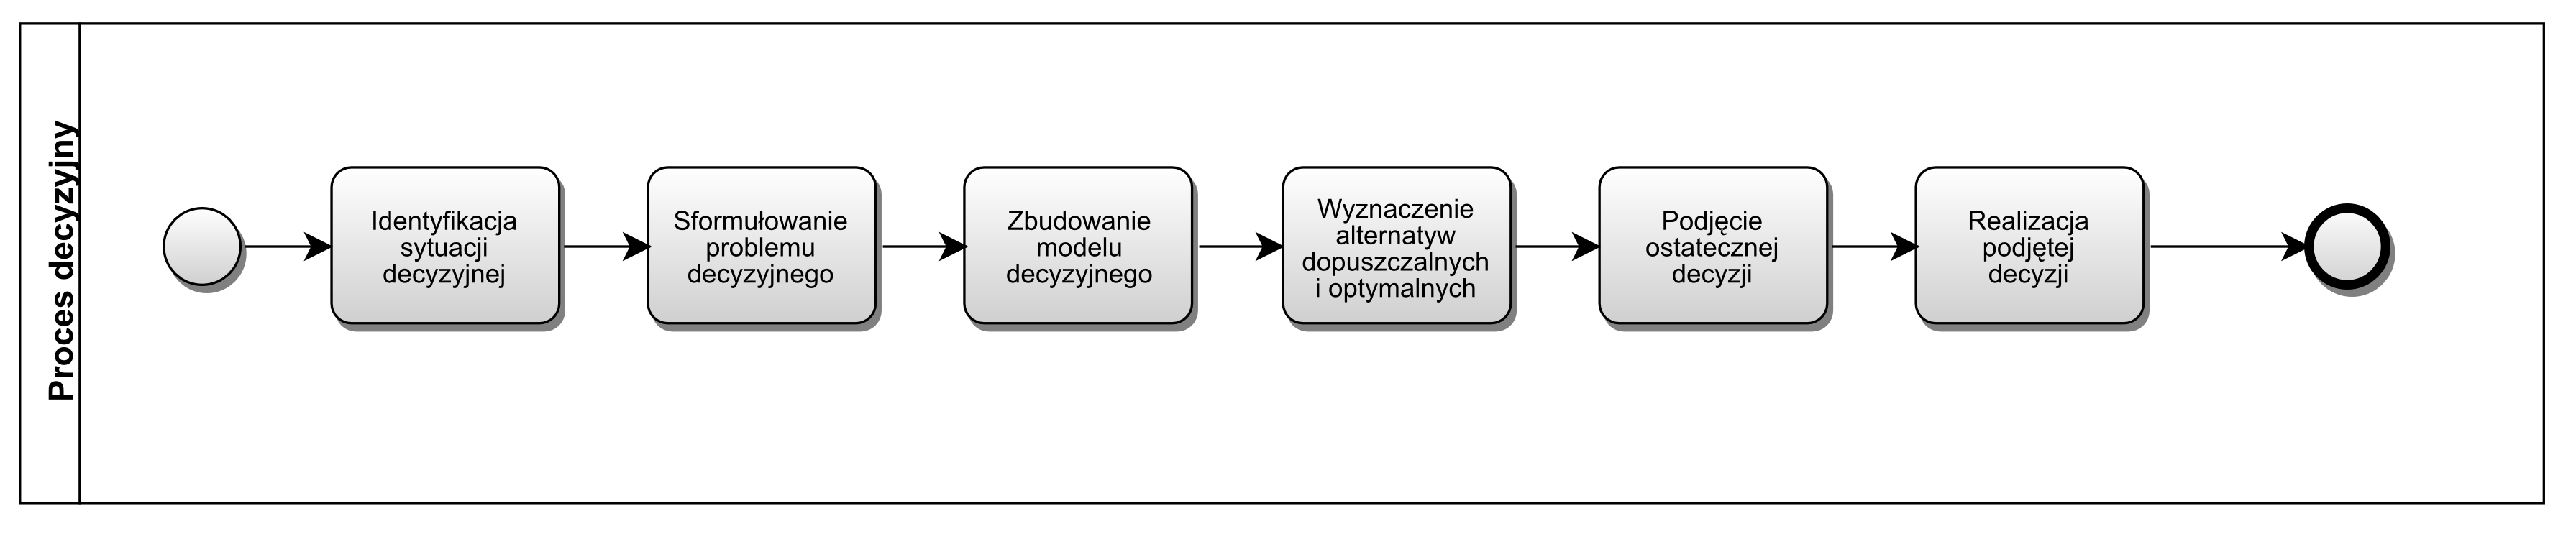
\includegraphics[width=\linewidth]
  {chapters/decisiontheory/proces_decyzyjny}
  \caption{Proces decyzyjny}
  \label{fig:proces_decyzyjny}
\end{figure}

\subsection{Metody}
Teoria decyzji nie jest jednolitą dziedziną nauki, a raczej zbiorem 
wypracowanych metod przez różne dziedziny. Omawiając metody stosowane w teorii 
decyzji, nie można zapominać o jej interdyscyplinarnym charakterze. Stosując 
modele matematyczne, jak na przykład metody programowania liniowego, nie 
powinno się przesłaniać psychologicznych i socjologicznych aspektów procesu 
decyzyjnego.

Metody podejmowania decyzji dzielone są na kategorie \cite{Fulop2005}. Jedną z
tych kategorii jest omówione wcześniej podejście normatywne. Jeżeli decyzja
podejmowana jest w warunkach pewności to mówi się o deterministycznych metodach
teorii decyzji, natomiast ryzykiem i niepewnością zajmują się metody
niedeterministyczne. Przypadkami kiedy jest więcej niż jedno kryterium oceny
decyzji, zajmuje się dział zwany wielokryterialną analizą decyzyjną.

Podejście deskryptywne jest kolejną kategorią metod teorii decyzji. Podejście 
deskryptywne zajmuje się opisem typowych zachowań ludzi w procesie decyzyjnym i 
wskazuje na czynniki mające wpływ na podjęcie ostatecznej decyzji. Dlatego 
wyróżnia się tutaj metody psychologiczne oraz socjologiczne, na przykład 
negocjacje.

Ważnym rodzajem metod teorii decyzji jest komputerowe wspomaganie decyzji. 
Rozwój technologii informatycznych spowodował, że systemy komputerowe zaczęły 
pełnić istotną rolę tam, gdzie trzeba przetworzyć szybko bardzo dużą ilość 
danych, wykorzystać skomplikowane obliczeniowo modele albo, w przypadku grup, 
nie ma możliwości spotkania się w jednym miejscu w jednym czasie.

\section{Interdyscyplinarność}
Nowoczesna teoria decyzji zaczęła się rozwijać od połowy dwudziestego wieku z 
wielu dyscyplin naukowych. Chociaż obecnie jest to w dużej części dziedzina 
ścisła, to zazwyczaj jest realizowana przez naukowców z zakresu ekonomii, 
psychologii, nauk politycznych i społecznych, socjologów i psychologów. 
Istnieją pewne podziały prac pomiędzy tymi grupami. Politolog będzie studiował 
zasady głosowania oraz inne aspekty grupowego podejmowania decyzji. Psycholog 
oraz socjolog może badać zachowania osób podejmujących decyzje, a filozof 
wymagania dotyczące racjonalności. Matematyk opisze cały proces w sposób 
formalny, a informatyk zbuduje system w oparciu o ten model.

Mimo szerokiego pola badań, istnieje duża zbieżność co do podejścia do problemu.
Naukowcy z różnych środowisk wykorzystują wyniki badań z wszystkich dziedzin i 
stosują je przy rozwiązywaniu tych samych lub podobnych problemów. Teorię 
decyzji można rozpatrywać pod kątem jednej dyscypliny niezależnie, jednak 
najlepsze wyniki, najbardziej zbliżone do rzeczywistości, uzyskiwane są po 
uwzględnieniu osiągnięć wszystkich dziedzin zajmujących się teorią decyzji.

